\chapter{Die Implementierung}

In diesem Kapitel wird auf die Implementierung des Simulators eingegangen. Der Simulator wurde in der Programmiersprache Java entwickelt. Bei der Betrachtung der Zielgruppe wird klar, dass Java f\"{u}r die gestellte Aufgabe die geigneste Programmiersprache ist. Der Simulator ist somit auf jeder Platform verf\"{u}gbar, f\"{u}r die es die JRE (Java Runtime Environment) gibt und erstreckt sich somit \"{u}ber alle g\"{a}ngigen Betriebssysteme. Da an der Fachhochschule Aachen auch Java gelehrt wird, sollten hier die meisten Studenten auch eigene Erweiterungen, wie eigene Protokolle, entwerfen k\"{o}nnen. Der Simulator wurde mit dem derzeit aktuellsten Java SDK (Software Development Kit) in der Version 6 (1.6) entwickelt.

\begin{table}
	\fbox{
	\begin{tabular}{l|l}
		\textbf{Paketname} & \textbf{Beschreibung} \\
		\hline 
		\textit{core} & Klassen f\"{u}r Prozesse und Nachrichten\\
		\textit{core.time} & Klassen f\"{u}r Zeitformate\\
		\textit{events} & Basisklassen f\"{u}r Ereignisse\\
		\textit{events.implementations} & Implementierungen von Ereignissen\\
		\textit{events.internal} & Implementierungen von internen Ereignissen\\
		\textit{exceptions} & Klassen f\"{u}r Fehlerbehandlungen\\
		\textit{prefs} & Klassen f\"{u}r die Einstellungen\\
		\textit{prefs.editors} & Klassen f\"{u}r die Editoren\\
		\textit{protocols} & Basisklassen f\"{u}r Protokolle\\
		\textit{protocols.implementations} & Implementierungen von Protokollen\\
		\textit{serialize} & Helferklassen f\"{u}r die Serialisierung von Simulationen\\
		\textit{simulator} & Klassen f\"{u}r die GUI und die Visualisierung\\
		\textit{utils} & Diverse Helferklassen\\
	\end{tabular}
	}
	\caption{Die Paketstruktur}
	\label{tb:Pakete}
\end{table}

Da es sonst den Rahmen sprengen w\"{u}rde, soll im Folgenden der komplette Quelltext nicht bis in das letzte Detail behandelt werden. Der Quelltext erstreckt sich n\"{a}mlich, einschlie�lich Kommentare, auf \"{u}ber 15.000 Zeilen und \"{u}ber 60 Dateien. Zudem ist die generierte Quelltext-Dokumentation (Javadoc) \"{u}ber 2MB gro�. Alle folgenden UML-Diagramme stellen aufgrund der \"{U}bersichtlichkeit lediglich die wesentlichen Dinge dar. Alle Details lassen sich im Quelltext und der dazugeh\"{o}rigen Dokumentation einsehen. Die Paketstruktur des Quelltextes ist in Tabelle \ref{tb:Pakete} in alphanumerischer Reihenfolge aufgef\"{u}hrt.  

\section{Programmierrichtlinien}

Die Programmierrichtlinien entsprechen in den meisten F\"{a}llen denen aus der Vorlesung \cite{OOS}. Die Main-Methode befindet sich in der Klasse \textit{simulator.VSMain}. 

\begin{itemize}
	\item Alle Klassen- und Interfacenamen beginnen mit gro�en Buchstaben, w\"{a}hrend alle Variablen-, Methoden- und Attributnamen mit kleinen Buchstaben beginnen. Namen statischer Variablen und Attribute sind komplett in Gro�buchstaben gehalten.
	\item Alle Quelltext-Dateien besitzen einen Header, der Informationen der verwendeten Lizenz angibt.
	\item Alle Quelltext-Dateien sind vollst\"{a}ndig mit Javadoc dokumentiert worden. 
	\item Der komplette Quelltext inklusive Dokumentation wurde in englischer Sprache verfasst. 
	\item Eine Quelltext-Datei hat eine maximale Zeilenl\"{a}nge von 80 Zeichen. Eine Ausnahme stellt die Klasse \textit{prefs.VSDefaultPrefs} dar, denn hier befinden sich auch l\"{a}ngere Texte die in Strings abgespeichert werden, wo manuelle Zeilenumbr\"{u}che wenig Sinn ergeben. 
	\item Es werden zuerst Klassen aus der Java-Standardbibliothek importiert, bevor Klassen aus dem VS-Simulator selbst importiert werden.
	\item F\"{u}r die Einr\"{u}ckung des Quelltextes wird das Tool \textit{astyle} mit den Aufrufparametern \textit{--style=java --mode=java} verwendet. Hierbei wird eine Einr\"{u}ckungsl\"{a}nge von 4 Zeichen verwendet.
	\item Namen abstrakter Klassen tragen stets das Prefix \textit{VSAbstract}.
	\item Namen aller Klassen und Interfaces tragen als Prefix stets \textit{VS}, was f\"{u}r Verteilte Systeme steht. 
\end{itemize}



\section{Einstellungen und Editoren}

Eine Simulation ist von einer Vielzahl von Einstellungen abh\"{a}ngig. Da auf diese Einstellungen in den weiteren Teilkapitel sets zur\"{u}ckgegriffen wird, macht es Sinn die dazugeh\"{o}rigen Klassen zuerst zu betrachten.

\subsubsection{Das Paket \textit{prefs}}

\begin{figure}[htbp]
	\centering
	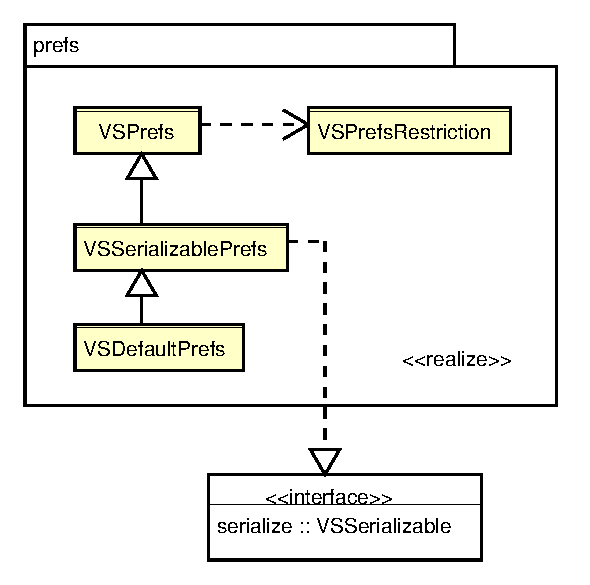
\includegraphics[width=7cm]{images/prefs}
	\caption{Das Paket \textit{prefs}}
	\label{fig:PackagePrefs}
\end{figure}

Auf Abbilung \ref{fig:PackagePrefs} ist der Aufbau des Pakets \textit{prefs} zu sehen. In einer Instanz der Klasse \textit{VSPrefs} lassen sich viele verschiedene Daten als Variablen f\"{u}r eine sp\"{a}tere Verwendung dynamisch ablegen und stellt somit einen Container f\"{u}r diese Daten dar. In einem \textit{VSPrefs}-Objekt speichert der Simulator alle seine Einstellungen ab. Zudem besitzt jedes Prozessobjekt und jedes Protokollobjekt f\"{u}r lokale Einstellungen seine eigene Instanz von \textit{VSPrefs}. Selbst Nachrichtenobjekte besitzt hiervon eine eigene Instanz, wobei hier die zu verschickenden Daten abgelegt werden k\"{o}nnen.

Jede Variable besteht aus einen Datentypen, einen Variablenamen und einer optionalen Beschreibung. Einige Datentypen unterst\"{u}tzen auch die Angabe von Minimum- und Maximumwerten (zum Beispiel besteht eine Prozentangabe aus einen Integerwert zwischen \textit{0} und \textit{100}), was mithilfe der \textit{VSPrefsRestriction}-Klasse implementiert wird. Da man beispielsweise bei Prozent ein \textit{\%} und bei Millisekunden ein \textit{ms} hinter der Variable sehen m\"{o}chte, kann f\"{u}r jede Variable auch ein optionaler Einheiten-String abgespeichert werden. Alle verf\"{u}gbaren Typen wurden bereits in Tabelle \ref{tb:VariablenDatentypen} aufgelistet. \textit{VSPrefs} stellt f\"{u}r alle Variablen entsprechende Zugriffsmethoden zur Verf\"{u}gung.  

Im Folgenden werden nicht alle exisierenden Methoden aufgelistet, da diese auch in der Quelltext-Dokumentation (Javadoc) eingesehen werden k\"{o}nnen. Die Methoden werden nun nur anhand des Integer-Datentyps verdeutlicht. F\"{u}r alle anderen Typen gilt fast alles analog. F\"{u}r Integer stehen in \textit{VSPrefs} folgende Methoden zur Verf\"{u}gung:

\begin{itemize}
	\setlength{\itemsep}{-2mm}
	\item \textit{void setInteger(String key, Integer val)}
	\item \textit{void setInteger(String key, Integer val, String descr)}
	\item \textit{void setInteger(String key, int val)}
	\item \textit{void setInteger(String key, int val, String descr)}
	\item \textit{Integer getIntegerObj(String key)}
	\item \textit{int getInteger(String key)}
	\item \textit{java.util.Set<String> getIntegerKeySet()}
	\item \textit{void initInteger(String key, int val) }
	\item \textit{void initInteger(String key, int val, String descr) }
	\item \textit{void initInteger(String key, int val, String descr, int minValue, int maxValue) }
	\item \textit{void initInteger(String key, int val, String descr, int minValue, int maxValue, String unit) }
	\item \textit{void initInteger(String key, int val, String descr, VSPrefsRestriction.VSIntegerPrefsRestriction r) }
	\item \textit{void initInteger(String key, int val, String descr, VSPrefsRestriction.VSIntegerPrefsRestriction r, String unit) }
\end{itemize}

Hierbei stellt \textit{key} den Variablennamen- und \textit{val} den Variablenwert dar. \textit{descr} ist eine optionale Variablenbeschreibung. Wenn f\"{u}r eine Variable keine Beschreibung existiert so wird, wie auf Abbildung \ref{fig:SimulationseinstellungenExperten} anhand der Farbvariablen schon gesehen wurde, f\"{u}r die Anzeige f\"{u}r eine Variable der Datentyp und der Variablenname verwendet. Es k\"{o}nnen sowohl Java's Integer-Objekte, als auch Java's primitiver Integer-Typ \textit{int} verwendet werden. Ein \textit{int}-Wert wird intern allerdings als Integer-Objekt abgespeichert und macht somit keinen gro�en Unterschied. Die Methode \textit{getIntegerKeySet} gibt alle vorhandenen Integer-Variablennamen (\textit{key}s) als \textit{Set} zur\"{u}ck.

\textit{VSPrefs} bietet auch eine Reihe von \textit{initInteger}-Methoden an, welche sich von den \textit{setInteger}-Methoden dadurch unterscheiden, dass sie eine Variable nur einen Wert zuweisen, wenn sie vorher noch nicht initialisiert wurde, was durch \textit{setInteger} oder \textit{initInteger} selbst geschehen sein kann. Eine komplette \"{U}bersicht aller Methoden (auch f\"{u}r andere Datentypen) gibt es in der Quelltext-Dokumentation.

\textit{VSPrefs} speichert alle Integervariablen in einem \textit{HashMap<String,Integer>}-Objekt ab, wobei der String-Wert den Variablenamen \textit{key} angibt. F\"{u}r die Beschreibung \textit{descr}, den Einheiten-String \textit{unit} sowie m\"{o}glichen Minimum- und Maximumwerte werden separate Instanzen von \textit{HashMap} verwendet. Da alle \textit{HashMap}-Objekte synchronisiert sind, k\"{o}nnen alle Methoden von verschiednenen Threads gleichzeitig verwendet werden. 

Die Klasse \textit{VSDefaultPrefs} erweitert \textit{VSPrefs} und initialisiert bei Instanzierung automatisch alle verf\"{u}gbaren Simulationsvariablen mit ihren Standardwerten. Dort sind auch alle Spracheinstellungen abgelegt. Sollte jemand den Simulator in eine andere Sprache, zum Beispiel ins Englische, \"{u}bersetzen wollen, so mu� er lediglich diese Datei und die Protokoll-Klassen (mehr dazu sp\"{a}ter) editieren. Die Spracheinstellungen sind n\"{a}mlich in einem \textit{VSPrefs}--Objekt als versteckte String-Variablen abgespeichert. Spracheinstellungen f\"{u}r Protokolle wurden in den Protokollklassen direkt angegeben, da dies mehr Komfort f\"{u}r den Protokollentwickler bietet und f\"{u}r jede neue Textausgabe nicht st\"{a}ndig \textit{VSDefaultPrefs.java} editiert werden muss. 

\begin{table}
	\fbox{
	\begin{tabular}{c|l|l}
		\textbf{Variablen-Prefix} & \textbf{Beschreibung}  & \textbf{Beispiel}\\
		\hline 
		\textit{col} & Farbvariablen & \textit{Color: col.background = Color-Objekt}\\
		\textit{div} & Diverse versteckte Variablen & \textit{Integer: div.window.loggsize = 300} \\
		\textit{keyevent} & Variablen, die Tastaturk\"{u}rzel definieren & \textit{Integer: keyevent.close = KeyEvent.VK\_C} \\
		\textit{lang} & Variablen, die Text beinhalten & \textit{String: lang.activate = aktivieren}\\
		\textit{message} & Variablen, die Nachrichten betreffen & \textit{Integer: message.prob.outage = 0}\\
		\textit{process} & Variablen, die Prozesse betreffen & \textit{Integer: process.prob.crash = 0}\\
		\textit{sim} & Allgemeine Simulationsvariablen & \textit{Integer: sim.process.num = 3}\\
	\end{tabular}
	}
	\caption{Konventionen f\"{u}r Variablennamen-Prefixe in \textit{VSDefautPrefs}}
	\label{tb:VariablenPrefixe}
\end{table}

Alle Variablen die als Prefix \textit{lang}, \textit{keyevent}, \textit{div} oder \textit{col} tragen, sind versteckte Variablen und werden in einem Editor nicht angezeigt. Im Expertenmodus sind hingegen nur Variablen die mit \textit{lang} und \textit{keyevent} beginnen versteckt. Somit lassen sich im Expertenmodus weitere Variablen vom Anwender editieren.

\subsubsection{Das Paket \textit{prefs.editors}}
\begin{figure}[htbp]
	\centering
	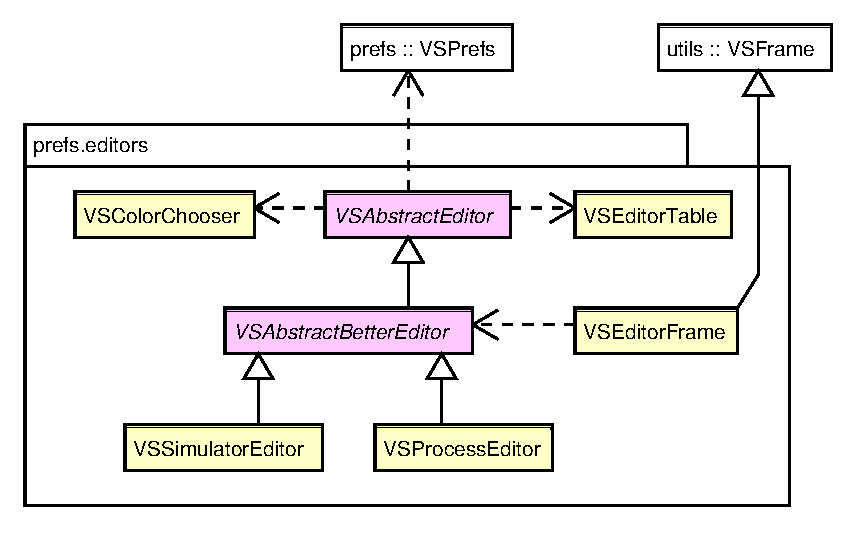
\includegraphics[width=11cm]{images/prefs-editors}
	\caption{Das Paket \textit{prefs.editors}}
	\label{fig:PackagePrefsEditors}
\end{figure}

Wie Variablen intern abgespeichert werden ist bereits bekannt. F\"{u}r das Editieren der Variablen werden Editor-Objekte verwendet. Auf Abbildung \ref{fig:PackagePrefsEditors} ist die Klassenstruktur des dazugeh\"{o}rigen Paketes \textit{prefs.editors} angegeben. 

Die Basis eines Editors stellt die abstrakte Klasse \textit{VSAbstractEditor} dar, dem ein \textit{VSPrefs} Objekt zum Editieren \"{u}bergeben wird. Ein Editor stellt alle verf\"{u}gbaren und nicht-versteckten Variablen des \textit{VSPrefs}-Objektes im GUI dar und bietet gleichzeitig die M\"{o}glichkeit alle Variablen dar\"{u}ber zu editieren an. F\"{u}r das Editieren von Farbwerten wird auf \textit{VSColorChooser} zur\"{u}ckgegriffen. Die Klasse \textit{VSEditorTable} ist f\"{u}r das \textit{JTable}-Objekt aus Java's Swing-Bibliothek zust\"{a}ndig, welches bei der graphischen Darstellung aller Variablen eingesetzt wird. Die abstrakte Klasse \textit{VSAbstractBetterEditor} wurde, wegen der \"{U}bersicht, als Zwischenschritt eingef\"{u}gt. 

Die Klasse \textit{VSSimulatorEditor} dient f\"{u}r das Editieren der globalen Simulationseinstellungen und \textit{VSProcessEditor} f\"{u}r das Editieren der Prozesseinstellungen sowie der dazugeh\"{o}rigen Protokollvariablen. Da diese beiden Klassen von \textit{VSAbstractBetterEditor} erben, k\"{o}nnen sie mithilfe von \textit{VSEditorFrame} in einem separaten Fenster angezeigt werden. Alternativ k\"{o}nnen die Editoren auch in der Sidebar im Tab ``Variablen'' angezeigt werden. Auf Abbildung \ref{fig:Simulationseinstellungen} wurde bereits ein \textit{VSEditorFrame} in Aktion gesehen.

F\"{u}r Protokolle gibt es keine separate Editor-Klasse, da sie bereits vom Prozesseditor aus editiert werden k\"{o}nnen. Dabei iteriert der Prozesseditor \"{u}ber alle f\"{u}r den jeweiligen Prozess verf\"{u}gbaren Protokollobjekte und f\"{u}gt deren Variablen zus\"{a}tzlich in den Prozesseditor ein. Somit erscheinen die Prozess- und die dazugeh\"{o}rigen Protokollvariablen im selben Editor, womit dem Benutzer eine bessere \"{U}bersicht geboten wird. 

\section{Ereignisse}

\subsection{Die Funktionsweise von Ereignissen}

F\"{u}r jedes Ereignis existiert eine dazugeh\"{o}rige Klasse, welche die auszuf\"{u}hrenden Aktionen implementiert. Eine Instanz davon wird, f\"{u}r eine sp\"{a}tere Ausf\"{u}hrung, in einem \textit{VSTask}-Objekt verpackt dem Task-Manager \"{u}bergeben. Auf den Task-Manager wird sp\"{a}ter noch genauer eingegangen. 
\begin{figure}[htbp]
	\centering
	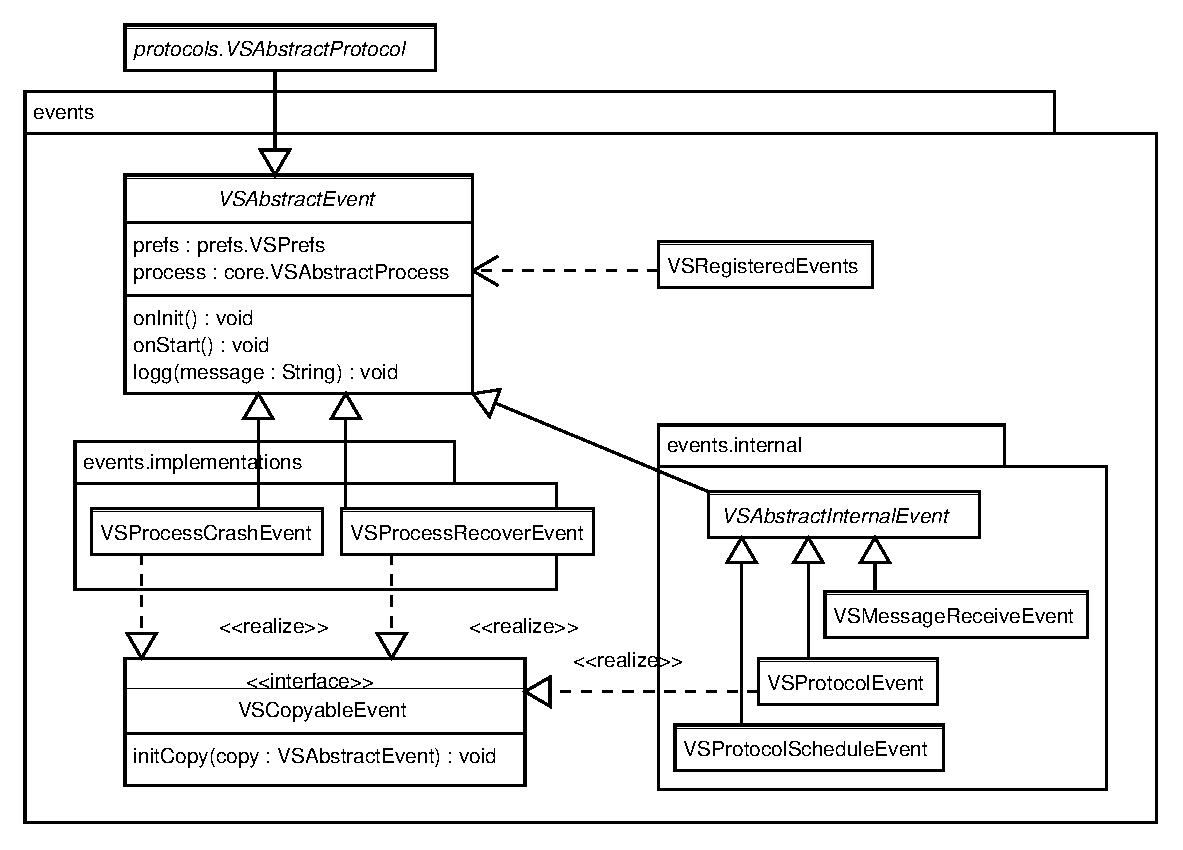
\includegraphics[width=13.5cm]{images/events}
	\caption{Die Pakete \textit{events} und \textit{events.*}}
	\label{fig:PackageEvents}
\end{figure}

Jedes programmierbare Ereignis mu�, bevor es vom Simulator verwendet werden kann, in der statischen Klasse \textit{VSRegisteredEvents} registriert werden. Da sich die Anzahl der verf\"{u}gbaren Ereignisse bei Laufzeit des Simulators nicht \"{a}ndert, gibt es keine Instanzen von \textit{VSRegisteredEvents}. Alle Methoden und Klassenattribute sind hier statisch. Wenn beispielsweise eigene Ereignisse implementiert werden, dann m\"{u}ssen alle neuen Ereignisse per Hand in die Datei \textit{VSRegisteredEvents.java} \"{u}bernommen- und der Simulator erneut kompiliert werden.

In der Implementierung wird zwischen drei Haupttypen von Ereignissen unterschieden, die jeweils in verschiedenen Paketen liegen:

\begin{enumerate}
	\item \textit{events.implementations}: In diesem Paket befinden sich alle Ereignisse, die ohne weitere Spezialbehanldung im Simulator eingesetzt werden k\"{o}nnen und vom Benutzer direkt im Ereigniseditor programmierbar sind. 
		\begin{itemize}
			\item \textit{VSProcessCrashEvent}: Dieses Ereignis l\"{a}sst den dazugeh\"{o}rigen Prozess abst\"{u}rzen.
			\item \textit{VSProcessRecoverEvent}: Dieses Ereignis l\"{a}sst den dazugeh\"{o}rigen Prozess wiederbeleben.
		\end{itemize}

	\item \textit{events.internal}: In diesem Paket befinden sich alle Ereignisse, die vom Simulator intern verwendet werden und dadurch eine direkte Programmierung via Ereigniseditor ausschlie�en. 		
		\begin{itemize}
			\item \textit{VSAbstractInternalEvent}: Diese Klasse stellt weitere Methoden zur Verf\"{u}gung, die von allen internen Ereignissen ben\"{o}tigt werden. Derzeit betrifft dies nur Methoden zur Serialisierung der gegebenen Objekte. Auf die Serialisierung (Abspeichern/Laden) von Simulationen wird sp\"{a}ter noch genauer eingegangen.
			\item \textit{VSMessageReceiveEvent}: Diese Klasse wird f\"{u}r die Ankunft einer Nachricht bei einem Empf\"{a}ngerprozess ben\"{o}tigt. Sie kapselt die eigentliche Nachricht und \"{u}berpr\"{u}ft, ob der Empf\"{a}ngerprozess das zur Nachricht dazugeh\"{o}rige Protokoll versteht. Diese Klasse \"{u}berpr\"{u}ft auch die Simulationseinstellung ``Nur relevante Nachrichten anzeigen'' und entscheidet, ob die Nachricht nach Eintreffen in der Visualisierung und im Loggfenster ber\"{u}cksichtigt werden soll oder nicht.
			\item \textit{VSProtocolEvent}: Diese Klasse implementiert gleichzeitig vier verschiedene Ereignisse: Das Aktivieren/Deaktivieren eines Servers/Clients eines gegebenen Protokolls. Der Ereigniseditor berechnet anhand der verf\"{u}gbaren Protokolle automatisch alle m\"{o}glichen Kombinationen und bietet sie dem Anwender in seiner Auswahl an. F\"{u}r alle dieser vier Ereignisse wird jeweils ein Objekt von \textit{VSProtocolEvent} verwendet, jedoch mit jeweils anderen Attributwerten.  
			\item \textit{VSProtocolScheduleEvent}: Diese Klasse wird f\"{u}r die Wecker-Ereignisse ben\"{o}tigt. Wecker-Ereignisse k\"{o}nnen nur von Protokollen (mehr dazu sp\"{a}ter) erstellt werden. \textit{VSProtocolScheduleEvent} besitzt eine Referenz auf das gegebene Protokoll und ruft bei Ereigniseintrittszeit entweder die Methode \textit{onServerScheduleStart} bei einem Server- oder \textit{onClientScheduleStart} bei einem Clientprotokoll auf. 
		\end{itemize}
	\item \textit{protocols.implementations}: In diesem Paket befinden sich alle Protokollimplementierung. Jedes Protokoll besitzt hier seine eigene Klasse. Alle Protokolle erben hierbei von der auf Abbildung \ref{fig:PackageEvents} zu sehenden Klasse \textit{protocols.VSAbstractProtocol}. Da \textit{protocols.VSAbstractProtocol} von \textit{events.VSAbstractEvent} erbt, kann ein Protokollobjekt auch als Ereignis eingesetzt werden. Ein solches Ereignis ruft bei Eintritt entweder die Methode \textit{onServerStart} oder die Methode \textit{onClientStart} des Protokolls auf, was einer Server- beziehungsweise einer Clientanfrage entspricht. Die Implementierung von Protokollen wird sp\"{a}ter genauer behandelt. 
\end{enumerate}

Alle Ereignisse, die das Interface \textit{VSCopyableEvent} implementieren, k\"{o}nnen vom Anwender im Ereigniseditor mit einem Rechtsklick kopiert werden und m\"{u}ssen die Methode \textit{initCopy(VSAbstractEvent copy)} implementieren. Dort werden alle relevanten Attribute in das neue Ereignis \textit{copy} kopiert. 

Alle Ereignisklassen erweitern die abstrakte Klasse \textit{VSAbstractEvent} und m\"{u}ssen folgende abstrakten Methoden implementieren:

\begin{itemize}
	\item \textit{abstract public void onInit()}: Bevor ein Ereignisobjekt vom Simulator verwendet werden kann, mu� es initialisiert werden. Je nach Ereignis k\"{o}nnen hier verschiedene Werte initialisiert werden. Diese Methode wird pro Ereignisobjekt nach Erstellung nur ein einziges Mal ausgef\"{u}hrt. 
	\item \textit{abstract public void onStart()}: Diese Methode wird jedes Mal ausgef\"{u}hrt, wenn das Ereignis eintritt. Sie stellt somit das Kernst\"{u}ck eines Ereignisses dar. 
\end{itemize}

Des Weiteren werden folgende nicht-abstrakte Methoden von \textit{VSAbstractEvent} vererbt:

\begin{itemize}
	\item \textit{public void logg(String message)}: Diese Methode schreibt eine Loggnachricht in das Simulationsloggfenster.
	\item \textit{public VSAbstractEvent getCopy()}: Diese Methode erstellt vom aktuellen Ereignis eine Kopie, wovon eine Referenz zur\"{u}ckgegeben wird. Alle Ereignisse die kopiert werden k\"{o}nnen m\"{u}ssen ebenso das Interface \textit{VSCopyableEvent} implementieren. Wenn ein Ereignis dies nicht tut und \textit{getCopy()} aufgerufen wird, dann wird von Java die Ausnahme \textit{exceptions.VSEventNotCopyable} geworfen.
	\item \textit{public VSAbstractEvent getCopy(VSInternalProcess process)}: Diese Methode erstellt vom aktuellen Ereignis ebenfalls eine Kopie, jedoch mit dem Unterschied, dass das Ereignis einem anderen Prozess zugewiesen wird. 
\end{itemize}

Jede Ereiginsklasse hat zudem Zugriff auf folgende Attribute, die von \textit{VSAbstractEvent} vererbt werden:

\begin{itemize}
	\item \textit{protected VSPrefs prefs}: Eine Referenz auf das Simulationseinstellungsobjekt. Hier\"{u}ber lassen sich alle Simulationseinstellungen beziehen.
	\item \textit{protected VSAbstractProcess process}: Eine Referenz auf das Prozessobjekt des jeweiligen Prozesses, auf welches das Ereignis angewendet wird.
\end{itemize}

\subsection{Beispielimplementierung eines Ereignisses}

Im Folgenden wird als Beispiel die Implementierung des Prozessabsturzereignisses \textit{VSProcessCrashEvent} behandelt. Da die dazugeh\"{o}rige Klasse keine Attribute besitzt, verleibt hier auch die \textit{initCopy}-Methode mit leerem Rumpf. Jede Ereignisklasse muss in \textit{onInit()} mit \textit{setClassname} den eigenen Klassennamen mitteilen. In \textit{onStart()} wird das eigentliche Ereignis ausgef\"{u}hrt. Hier wird obligatorisch \"{u}berpr\"{u}ft, ob der Prozess bereits abgest\"{u}rzt (hier eigentlich nicht Notwendig, verbessert aber die Lesbarkeit der Logik) ist und gegebenenfalls wird der Prozess dann zum Absturz bewegt. Der Task-Manager \"{u}berpr\"{u}ft bereits, ob der Prozess abgest\"{u}rzt ist oder nicht, d.h. ein Ereignis wird bei einem abgest\"{u}rztem Prozess gar nicht erst ausgef\"{u}hrt. Die einzige Ausnahme bildet ein Wiederbelebungsereignis (\text{VSProcessRecover}), welches vom Task-Manager ausgef\"{u}hrt wird, auch wenn der Prozess abgest\"{u}rzt ist. Mit \textit{logg} wird eine Nachricht in das Loggfenster geschrieben, welche ueber das \textit{VSPrefs}-Objekt \textit{prefs} bezogen wird:
\begin{code}
package events.implementations;

import events.*;

public class VSProcessCrashEvent 
extends VSAbstractEvent implements VSCopyableEvent {
    private static final long serialVersionUID = 1L;

    public void initCopy(VSAbstractEvent copy) {
    }

    public void onInit() {
        setClassname(getClass().toString());
    }

    public void onStart() {
        if (!process.isCrashed()) {
            process.isCrashed(true);
            logg(prefs.getString("lang.crashed"));
        }
    }
}
\end{code}

\section{Zeitformate, Prozesse, Nachrichten sowie Task-Manager}

\subsection{Funktionsweise}

Das Paket \textit{core.time} auf Abbildung \ref{fig:PackageCoreTime} stellt lediglich die Klassen f\"{u}r die Vektor- und Lamportzeitstempel zur Verf\"{u}gung. F\"{u}r die normale lokale Prozesszeit wird aus Performancegr\"{u}nden keine eigene Klasse, sondern ein einfaches \textit{long}-Attribut des Prozessobjektes verwendet.

\begin{figure}[htbp]
	\centering
	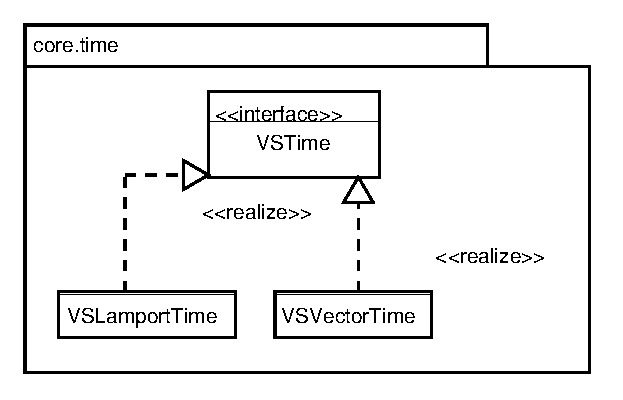
\includegraphics[width=7cm]{images/core-time}
	\caption{Das Paket \textit{core.time}}
	\label{fig:PackageCoreTime}
\end{figure}

Auf Abbildung \ref{fig:PackageCore} ist stark vereinfacht (in Wirklichkeit existieren in den angegebenen Klassen viel mehr Attribute und Methoden) das Paket \textit{core} dargestellt. F\"{u}r jedes auszuf\"{u}hrendes Ereignis wird eine Instanz von \textit{VSTask} ben\"{o}tigt, welche die Ereigniseintrittszeit als Attribut abgespeichert hat sowie eine Referenz auf das Objekt des auszuf\"{u}hrenden Ereignisses (\textit{VSAbstractEvent}) und dem Prozessobjekt besitzt. Geplante \textit{VSTask}-Instanzen werden f\"{u}r eine sp\"{a}tere Ausf\"{u}hrung dem Task-Manager \"{u}bergeben.

Die Kapselung eines \textit{VSAbstractEvent}-Objektes in einem \textit{VSTask}-Objekt erlaubt es, dass die selbe \textit{VSAbstractEvent}-Instanz mehrmals auf einmal im Task-Manager geplant werden kann. Ohne dieser Kapselung g\"{a}be es f\"{u}r jedes Ereignis lediglich nur eine einzige m\"{o}gliche Eintrittszeit. Von dieser M\"{o}glichkeit wird zum Beispiel bei den Server- und Clientanfragen eines Protokollobjektes Gebrauch gemacht. F\"{u}r jedes Protokoll kann der Anwender in einer Simulation beliebig viele Anfragen programmieren, wobei f\"{u}r jede Anfrage stets das selbe Protokollobjekt als Ereignis verwendet wird.

Jede Simulation besitzt genau eine Instanz von \textit{VSTaskManager}. Eine Instanz dieser Klasse stellt den Task-Manager dar. Er verwaltet alle \textit{VSTask}-Instanzen und \"{u}berpr\"{u}ft periodisch, ob es auszuf\"{u}hrende Ereignisse gibt. Der Task-Manager unterscheidet zwischen globalen und lokalen Ereignissen. Hierbei werden alle globalen Ereignisse (gekapselt in einem \textit{VSTask}-Objekt) in einer Priorit\"{a}ts-Warteschlange abgelegt. Die Priorit\"{a}ts-Warteschlange stellt hierbei die korrekte Ereigniseintrittsreihenfolge sicher. Da sich die lokalen Zeiten aller beteiligten Prozesse voneinander unterscheiden k\"{o}nnen, muss f\"{u}r jeden Prozess eine separate lokale Priorit\"{a}ts-Warteschlange verwendet werden, auf die jedes Prozessobjekt seine eigene Referenz hat. In den lokalen Warteschlangen sind die geplanten lokalen Ereignisse (auch gekapselt in einem \textit{VSTask}-Objekt) abgelegt. Der Task-Manager greift \"{u}ber eine \textit{java.util.ArrayList} auf alle Prozessobjekte zu und kann somit auch auf alle lokalen Warteschlangen zugreifen und diese verwalten.

\begin{figure}[htbp]
	\centering
	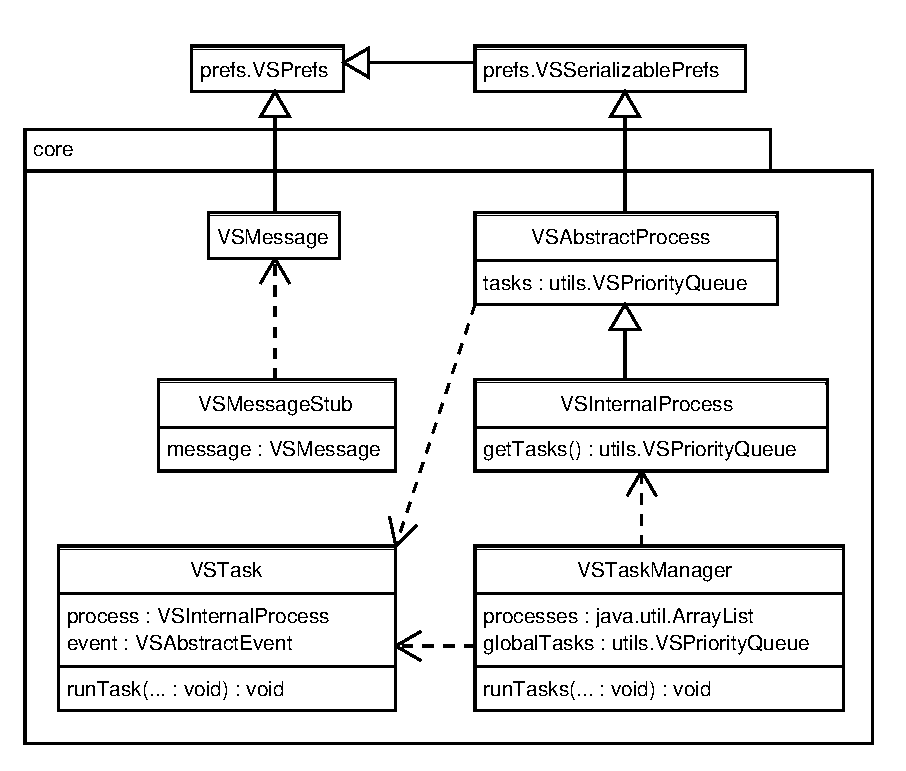
\includegraphics[width=10.0cm]{images/core}
	\caption{Das Paket \textit{core}}
	\label{fig:PackageCore}
\end{figure}

Eine Instanz von \textit{VSMessage} stellt eine Nachricht dar, die von einem Prozess verschickt wird. F\"{u}r jedes Versenden einer Nachricht wird hiervon eine Instanz gebildet, wo der Senderprozess die zu verschickende Daten ablegt. Da \textit{VSMessage} von \textit{VSPrefs} erbt, k\"{o}nnen zwischen zwei Prozessen beliebige Datentypen (Tabelle \ref{tb:VariablenDatentypen}) \"{u}ber eine Nachricht verschickt werden. Anschlie�end wird f\"{u}r jeden Empf\"{a}ngerprozess das neues Ereignisobjekt der Klasse \textit{VSMessageReceiveEvent} angelegt, welche eine Referenz der verschickten Nachricht besitzt. Danach wird ein \textit{VSTask}-Objekt instanziert, wo die Referenz auf das Ereignisobjekt und das dazugeh\"{o}rige Prozessobjekt sowie die Ereigniseintrittszeit als Attribute gespeichert werden. Das \textit{VSTask}-Objekt wird dann dem Task-Manager "{u}bergeben, der das dazugeh\"{o}rige Ereignis ausf\"{u}hrt, wenn die Ereigniseintrittszeit eingetroffen ist. 

Via Java-Polymorphie wird das \textit{VSMessageReceiveEvent}-Objekt in ein \textit{VSAbstractEvent} umgewandelt. Die dazugeh\"{o}rige Ereigniseintrittszeit $t_e$ wird jeweils wie folgt bestimmt:

\begin{equation*}
	t_e := TODO
\end{equation*}

Erw\"{a}hnentswert ist auch die Klasse \textit{VSMessageStub}, welche ein \textit{VSMessage} kapselt. Ihr Zweck ist das Verstecken einiger Methoden von \textit{VSMessage} im Protokoll-API, welches f\"{u}r die Erstellung eigener Protokolle dient. Der Protokoll-Entwickler soll m\"{o}glichst nichts falsch machen k\"{o}nnen und deswegen soll den Protokoll-API ein eingeschr\"{a}nkter Funktionsumpfang zur Verf\"{u}rung gestellt werden. Da sich \textit{VSMessageStub} im selben Paket wie \textit{VSMessage} befindet, kann \textit{VSMessageStub} auf paket-private Methoden (diejenigen Methoden, die weder als \textit{private}, \textit{protected} noch \textit{public} gekennzeichnet sind) von \textit{VSMessage} zugreifen. Protokolle hingegen werden in einem anderen Paket implementiert und haben somit keinen Zugriff auf diese paket-privaten Methoden. Zwar kann der Protokollentwickler ein eigenes \textit{VSMessageStub}-Objekt anlegen, jedoch kann er auf diese Weise besser unterscheiden, auf welche Mehhoden er zugreifen sollte und auf welche nicht. Das Protokoll-API wird sp\"{a}ter genauer behandelt. 

Der Task-Manager speichert anschlie�end die Empfangsereignisse in den lokalen Warteschlangen der Empf\"{a}ngerprozesse. Die Nachricht kommt bei einem Empf\"{a}ngerprozess an, sobald das Ereignis f\"{u}r den Empfang eintritt. F\"{u}r die korrekte Implementierung der Lamport- und Vektor-Zeitstempel wird jeder Nachricht automatisch eine Referenz auf die Lamport- sowie auf die Vektorzeit des sendenden Prozesses als Attribut beigef\"{u}gt. F\"{u}r die \"{U}berpr\"{u}fung des Protokolls wird in jeder Nachricht auch der Klassenname des jeweiligen Protokolls abgespeichert.

Eine Instanz von \textit{VSInternalProcess} repr\"{a}sentiert einen simulierten Prozess. Ein \textit{VSInternalProcess} stellt alle vom Simulator intern verwendeten Methoden zur Verf\"{u}gung, w\"{a}hrend ein \textit{VSAbstractProcess} lediglich Methoden hat, die man im Protokoll-API f\"{u}r die Erstellung eigener Protokolle verwenden darf. Da \textit{VSAbstractProcess} abstrakt ist und hiervon keine Instanz gebildet werden darf, muss f\"{u}r einen neuen Prozesses stets ein \textit{VSInternalProcess}-Objekt erstellt werden. Via Polymorphie wird dieses Objekt nach \textit{VSAbstractProcess} umgewandelt und so dem Protokoll-API zur Verf\"{u}gung gestellt. Beispielsweise darf mit \textit{getTasks()} nur vom Simulator intern auf die Priorit\"{a}ts-Warteschlangen zugegriffen werden, w\"{a}hrend man im Protokoll-API selbiges vermeiden sollte und auch gar nicht direkt m\"{o}glich ist. Hierf\"{u}r h\"{a}tte man auch ein Stub-Objekt \textit{VSProcessStub} verwenden k\"{o}nnen. Da aber so gut wie alle paar Millisekunden auf die Methoden von \textit{VSInternalProcess} zugegriffen wird, wurde hier aus Performancegr\"{u}nden der Weg \"{u}ber eine Vererbungungsstufe preferiert. 

Alle einstellbaren Prozessvariablen werden von der Klasse \textit{VSPrefs} vererbt. Damit bei Neuberechnungen die Variablen nicht dauernd \"{u}ber eine \textit{HashMap} von \textit{VSPrefs} zugregriffen werden mu�, speichert \textit{VSInternalProcess} aus Performancegr\"{u}nden einige Variablen als lokale Kopie ab. Zum Beispiel wird f\"{u}r die lokale Prozesszeit nicht auf das \textit{HashMap<String,Long>}-Objekt von \textit{VSPrefs}, sondern auf das Klassenattribut \textit{private long localTime} zugegriffen. Vor- und nach dem Editieren \"{u}ber den Prozesseditor werden die \textit{VSPrefs} beziehungsweise die lokalen Kopien auf den neusten Stand gebracht. Selbiges gilt f\"{u}r weitere Variablen wie zum Beispiel der Uhrabweichung eines Prozesses.

\subsection{Beispiel f\"{u}r die Erstellung von Prozessereignissen}

Anhand der Prozessabsturz- und Wiederbelebungsereignisse l\"{a}�t sich wie folgt sehr gut demonstieren, wie intern Ereignisse angelegt werden k\"{o}nnen:
\begin{code}
void createCrashAndRecoverExample(VSTaskManager taskManager,
                                  VSInternalProcess process) {
    VSAbstractEvent crashEvent = new VSProcessCrashEvent();
    VSTask localTask = new VSTask(process.getTime()+500, process, 
                                  crashEvent, VSTask.LOCAL);
    taksManager.addTask(localTask);

    VSAbstractEvent recoverEvent = new VSProcessRecoverEvent();
    VSTask globalTask = new VSTask(2000, process, 
                                  recoverEvent, VSTask.GLOBAL);
    taksManager.addTask(globalTask);
}
\end{code}

In diesem Beispiel wurden zwei Ereignisse (Absturz- und Wiederbelebung eines gegebenen Prozesses) angelegt. Das Absturzereignis tritt bei der aktuellen lokalen Prozesszeit plus \textit{500ms} ein, w\"{a}hrend das Wiederbelebungsereignis bei einer globalen Zeit von \textit{2000ms} stattfindet. F\"{u}r den Fall, dass das Wiederbelebungsereignis vor dem Absturzereignis eintritt, wird es nicht ausgef\"{u}hrt, da der Prozess noch nicht abgest\"{u}rzt ist. 

\section{Protokolle}

\subsection{Die Funktionsweise des Protokoll-APIs}

\begin{figure}[htbp]
	\centering
	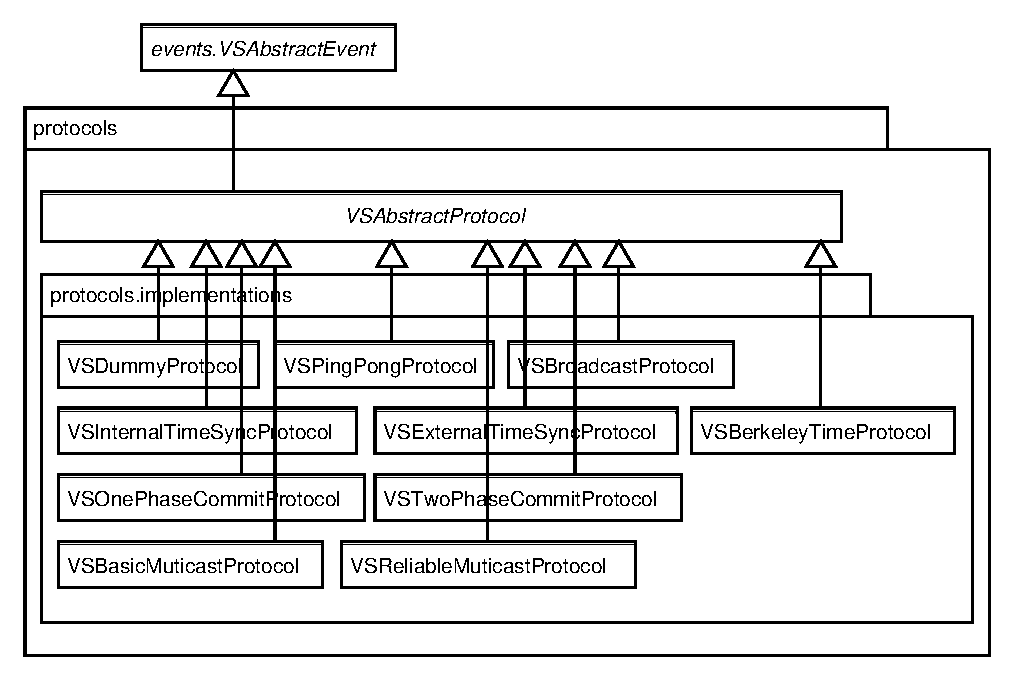
\includegraphics[width=12cm]{images/protocols}
	\caption{Die Pakete \textit{protocols} und \textit{protocols.*}}
	\label{fig:PackageProtocols}
\end{figure}

In diesem Abschnitt wird auf die Implementierung der Protokolle eingegangen. Auf Abbildung \ref{fig:PackageProtocols} sind die Pakete \textit{protocols} und \textit{protocols.implementations} dargestellt, welche f\"{u}r die Protokollimplementierungen zust\"{a}ndig sind. \textit{VSAbstractProtocol} stellt lediglich gemeinsame Methoden und Attribute zur Verf\"{u}gung, die von allen Protokollen verwendet werden k\"{o}nnen. Jedes Protokoll hat im Paket \textit{protocols.implementations} seine eigene Klasse, die von \textit{VSAbstractProtocol} erbt. Wie bereits erw\"{a}hnt erbt \textit{VSAbstractProtocol} von \textit{VSAbstractEvent}, sodass jedes Protokoll auch als Ereignis (Server- beziehnungsweise Clientanfrage starten) eingesetzt werden kann.

Jede Protokollklasse mu� die folgenden Methoden implementieren:

\begin{itemize}
	\item Einen \"{o}ffentlichen (\textit{public}) Konstruktor. Der Konstruktor mu� angeben, ob bei dem gegebene Protokoll der Client oder der Server die Anfragen startet. 
	\item \textit{abstract public void onClientInit()}: Bevor das Protokollobjekt benutzt werden kann, mu� es initialisiert werden. Diese Methode wird vor dem ersten Verwenden des Protokolls innerhalb einer Simulation ausgef\"{u}hrt. In der Regel werden hier Protokollvariablen unter Verwendung von \textit{VSPrefs} und Attribute der Protokollklasse initialisiert. Die hier initialisierten Protokollvariablen lassen sich vom Benutzer im Prozesseditor des jeweiligen Prozesses editieren.
	\item \textit{abstract public void onClientReset()}: Dese Methode wird jedes Mal ausgef\"{u}hrt, wenn die Simulation zur\"{u}ckgesetzt wird.
	\item \textit{abstract public void onClientStart()}: Diese Methode wird nur ben\"{o}tigt, wenn der Client immer die Anfragen startet. Diese Methode generiert in der Regel immer eine Clientanfrage, die via \textit{VSMessage}-Objekt an alle beteiligten Prozesse verschickt wird.
	\item \textit{abstract public void onClientRecv(VSMessage message)}: Diese Methode wird jedes Mal Ausgef\"{u}hrt, wenn eine Servernachricht \textit{message} bei dem Client eintrifft. 
	\item \textit{abstract public void onClientSchedule()}: Diese Methode wird jedes Mal ausgef\"{u}hrt, wenn ein Wecker-Ereignis eintritt. 
	\item \textit{public String toString()}: Diese Methode ist nur optional. Hiermit lassen sich die Loggnachrichten eines Protokolls anpassen. Wenn diese Methode in einer Protokollimplementierung ausgelassen wird, so wird stets die \textit{toString}-Methode der Mutterklasse \textit{VSAbstractProtocol} verwendet.
\end{itemize}

F\"{u}r alle hier aufgelisteten Client-Methoden sind auch die korespondierenen Server-Methoden anzugeben. Die Server-Methoden sind analog zu den Client-Methoden aufgebaut. 

\subsection{Beispielimplementierung eines Protokolls}

Im Folgenden wird die Implementierung des zuverl\"{a}ssigen Multicast-Protokolls \textit{VSReliableMulticastProtocol.java} als Beispiel aufgef\"{u}hrt. Die Funktionsweise des Protokolls wurde bereits in Kapitel 2.5.10 beschrieben. Client- und Serverseite werden in der selben Klasse implementiert.

Im Konstruktor mu� stets angegeben werden, ob beim gegebenen Protokoll der Client oder der Server die Anfragen startet. Mit \textit{HAS\_ON\_CLIENT\_START} wird dem API mitgeteilt, dass der Client die Anfragen startet. F\"{u}r \textit{HAS\_ON\_SERVER\_START} und Serveranfragen gilt Selbiges analog:
	
\begin{code}
package protocols.implementations;

import java.util.ArrayList;
import java.util.Vector;
import protocols.VSAbstractProtocol;
import core.VSMessage;

public class VSReliableMulticastProtocol 
	extends VSAbstractProtocol {
    public VSReliableMulticastProtocol() {
        super(VSAbstractProtocol.HAS_ON_CLIENT_START);
        setClassname(getClass().toString());
    }
\end{code}

\subsubsection{Clientseite des Protokolls}

Das private Klassenattribut \textit{pids} wird f\"{u}r die Zwischenspeicherung beteiligter PIDs ben\"{o}tigt. Hier sind alle PIDs abgelegt, von denen noch Best\"{a}tigungsnachrichten erwartet werden. Hier werden als Standard-PIDs \textit{1} und \textit{3} verwendet. Die Methoden \textit{initVector} und \textit{initLong} wurden von \textit{VSPrefs} vererbt und initialisieren die Protokollvariablen \textit{pids} und \textit{timeout}, welche vom Benutzer im Prozesseditor editiert werden k\"{o}nnen:
\begin{code}
    private ArrayList<Integer> pids;

    public void onClientInit() {
        Vector<Integer> vec = new Vector<Integer>();
        vec.add(1); vec.add(3);
        initVector("pids", vec, "PIDs beteilitger Prozesse");
        initLong("timeout", 2500, 
                 "Zeit bis erneute Anfrage", "ms");
    }
\end{code}

Wenn die Simulation zur\"{u}ckgesetzt wird, dann wird auch \textit{pids} reinitialisiert:
\begin{code}
    public void onClientReset() {
       	pids.clear();
        pids.addAll(getVector("pids"));
    }
\end{code}

In \textit{onClientStart} wird gepr\"{u}ft, ob eine Clientanfrage gestartet werden soll. Wenn dies der Fall ist (wenn von mindestens einem beteiligten Prozess noch keine Best\"{a}tigung erhalten wurde), wird ein neues Nachrichtenobjekt erstellt, und mit dem Inhalt \textit{Boolean: isMulticast=true} verschickt (intern wird hier f\"{u}r jeden Empf\"{a}ngerprozess ein \textit{VSMessageReceiveEvent} erzeugt). Mit \textit{scheduleAt} wird ein Wecker festgelegt, zur welchen lokalen Prozesszeit die Methode \textit{onClientSchedule} aufgerufen werden soll (intern wird hier ein \textit{VSProtocolScheduleEvent} erzeugt): 
\begin{code}
    public void onClientStart() {
        if (pids.size() != 0) {
            long timeout = getLong("timeout") + process.getTime();
            scheduleAt(timeout);

            VSMessage message = new VSMessage();
            message.setBoolean("isMulticast", true);
            sendMessage(message);
        }
    }
\end{code}

Wenn eine Serverantwort eintrifft, dann wird \textit{onClientRecv} aufgerufen. Hier wird \"{u}berpr\"{u}ft, ob \"{u}berhaupt noch Multicast-Best\"{a}tigungen ben\"{o}tigt werden. Wenn dies der Fall ist, dann wird geschaut, ob es sich bei der Antwort um eine noch nicht eingetroffene Best\"{a}tigung handelt. Gegebenenfalls wird die jeweilige PID aus \textit{pids} entfernt. Wenn \textit{pids} leer ist, dann wurde von allen beteiligten Prozessen eine Best\"{a}tigung erhalten und der Client entfernt mit \textit{removeSchedules} alle seine derzeit programmierten Wecker.

\begin{code}
    public void onClientRecv(VSMessage recvMessage) {
        if (pids.size() != 0 && recvMessage.getBoolean("isAck")) {
            Integer pid = recvMessage.getIntegerObj("pid");

            if (pids.contains(pid)) 
                pids.remove(pid);
            else 
                return;

            logg("ACK von Prozess " + pid + " erhalten!");

            if (pids.size() == 0) {
                logg("ACKs von allen beteiligten Prozessen " +
                     "erhalten!");

                removeSchedules();
            }
        }
    }
\end{code}

F\"{u}r das erneute Verschicken einer Clientanfrage ruft \textit{onClientSchedule} lediglich die Methode \textit{onClientStart} auf, die wiederum einen neuen Wecker planen kann:
\begin{code}
    public void onClientSchedule() {
        onClientStart();
    }
\end{code}

\subsubsection{Serverseite des Protokolls}

Die Serverseite des Protokolls speichert im Attribut \textit{ackSent} ab, ob es bereits eine Best\"{a}tigung des Multicasts verschickt hat oder nicht. In diesem Protokoll werden in \textit{onServerInit} keine Initialisierungen vorgenommen. Demach gibt es f\"{u}r den Benutzer auch keine serverseitigen Protokollvariablen zu editieren. Beim Zur\"{u}cksetzen der Simulation wird lediglich \textit{ackSent} auf den Ursprungswert gesetzt:
\begin{code}
    private boolean ackSent;

    public void onServerInit() { }

    public void onServerReset() {
        ackSent = false;
    }
\end{code}

Wenn der Server eine Clientanfrage erhalten hat, so \"{u}berpr\"{u}ft der Server, ob es sich um eine Multicast-Nachricht handelte. Anschlie�end wird gegebenenfalls die Best\"{a}tigungsnachricht mit \textit{Boolean: isAck=true} und der Server-PID verschickt. Jenachdem ob bereits eine Best\"{a}tigung verschickt wurde oder nicht wird eine andere Nachricht geloggt: 
\begin{code}
    public void onServerRecv(VSMessage recvMessage) {
        if (recvMessage.getBoolean("isMulticast")) {
            VSMessage message = new VSMessage();
            message.setBoolean("isAck", true);
            message.setInteger("pid", process.getProcessID());
            sendMessage(message);

            if (ackSent) {
                logg("ACK erneut versendet");
            } else {
                logg("ACK versendet");
                ackSent = true;
            }
        }
    }
\end{code}

Der Server benutzt in diesem Beispiel keinen Wecker. Dementsprechend hat die Methode \textit{onServerSchedule} auch einen leeren Rumpf:
\begin{code}
    public void onServerSchedule() { }
}
\end{code}

\subsection{Erstellung eigener Protokolle}

\section{GUI}

\section{Serialisierung von Simulationen}

\subsection{R\"{u}ckw\"{a}rtskompatibel}

\section{Weiteres}

exceptions, utils

\section{Entwicklungsumgebung}

In diesem Teilkapitel soll ein kleiner Einblick in die Umgebung, in der der Simulator entwickelt wurde, gew\"{a}hrt werden. F\"{u}r diese Diplomarbeit wurde ausschlie�lich Open Source Software verwendet. Die einzige Ausnahme stellt Microsoft Windows XP dar, worauf der Simulator zus\"{a}tzlich getestet wurde. Der Simulator wurde jedoch haupts\"{a}chlich unter dem Betriebssystem FreeBSD 7.0, was ein open source Unix-Derivat ist, programmiert. 

Wie bereits bekannt ist, wurde Sun's Java, was mittlerweile auch Open Source Software ist, in der Version 6 (1.6) als die Implementierungssprache gew\"{a}hlt und f\"{u}r die Quelltextdokumentation kam Javadoc und f\"{u}r die automatische Quelltexteinr\"{u}ckung astyle zum Einsatz. Als Built-Tool wurde hier auf Apache Ant gesetzt. F\"{u}r die Erstellung dieses PDF-Dokumentes wurde LaTeX in Verbindung mit dem Built-Tool GNU Make und Rubber verwendet. Eine Rechtschreib\"{u}berpr\"{u}fung wurde mit aspell durchgef\"{u}hrt. xPDF diente als PDF-Anzeigeprogramm.

Als Versionierungssystem wurde SVN (Subversion) verwendet. F\"{u}r den Zugriff auf das SVN-Repository mittels HTTPS (Hypertext Transfer Protocol Secure) wurde der Apache-Websever mit WebDAV-Plugin verwendet. Zudem kam WebSVN als Webschnitstelle des SVN-Repositories zum Einsatz. Als SSL Zertifikat diente ein Kostenloses von CaCert (\url{http://www.CaCert.org}). Mozilla Firefox diente f\"{u}r das Betrachten der Javadocs und der WebSVN-Oberfl\"{a}che.

F\"{u}r schreiben von Java-Quelltext wurde GVim (Graphical Vi IMproved) sowie Eclipse verwendet. Eclipse unterst\"{u}tzt bessere Code-Refactoring-Methoden, w\"{a}hrend GVim mit seiner Flexibilit\"{a}t und schnelleren Editierm\"{o}glichkeiten und mit Vim-Script, der eigenen Script-Engine, gl\"{a}nzt. Es wurden ausserdem das JAutoDoc- (f\"{u}r die Erstellung von Javadoc-Kommentate) und das Subversion-Eclipse-Plugin verwendet. Je nach Zweck wurde zwischen diesen beiden Umgebungen gewechselt. F\"{u}r das Verfassen des LaTeX-Dokumentes wurde GVim verwendet.

S\"{a}mtliche UML-Diagramme wurden mit ArgoUML angefertigt und die Screenshots mit The GIMP (GNU Image Manipulation Program) sowie ImageMagick nachbearbeitet. Mit zip wurden alle VS-Simulator Distributionen eingepackt.

\subsubsection{Linkliste der verwendeten Software}

\begin{itemize}
	\setlength{\itemsep}{-2mm}
	\item Apache Webserver - \url{http://httpd.apache.org}	
	\item ArgoUML - \url{http://argouml.tigris.org}
	\item Eclipse - \url{http://www.eclipse.org}
	\item FreeBSD - \url{http://www.FreeBSD.org}
	\item GNU Make - \url{http://www.gnu.org/software/make}
	\item GVim - \url{http://www.vim.org}
	\item ImageMagick - \url{http://www.imagemagick.org}
	\item Javadoc - \url{http://java.sun.com/j2s2/javadoc}
	\item Mozilla Firefox - \url{http://www.mozilla.com}
	\item Rubber - \url{http://www.pps.jussieu.fr/~beffara/soft/rubber}
	\item Sun Java - \url{http://java.sun.com}
	\item The GIMP - \url{http://www.gimp.org}
	\item WebDAV - \url{http://httpd.apache.org/docs/2.0/mod/mod\_dav.html}	
	\item WebSVN - \url{http://websvn.tigris.org}
	\item aspell - \url{http://aspell.sourceforge.net}
	\item astyle - \url{http://astyle.sourceforge.net}
	\item xPDF - \url{http://www.foolabs.com/xpdf}
	\item zip - \url{http://www.info-zip.org/Zip.html}
\end{itemize}

